\section{仿射限制}\label{sec:affine-restrictions}

为了把射影簇与更容易画出图形的仿射簇联系起来, 回顾 Section~\ref{sec:projective-space} 中射影空间的第二种视角: 把 $\mathbb{P}^{n}$ 看成向 $\mathbb{A}^{n}$ 添加无穷远点得到的空间. 略去这些无穷远点, 就能为每个射影簇找到一个仿射限制. 这种限制为我们提供了射影簇的一幅有用但不完整的图景. 在解释一般概念前, 先看一个具体例子.

\begin{Example}{$\mathbb{P}^{2}$ 中一条二次曲线的仿射限制}\leavevmode\label{ex:affine-restriction-of-projective-conic}
\BookPairedNote
  {考虑射影簇
  \[
    X=\mathcal{V}_{\mathbb{P}}(x_{0}^{2}+x_{1}^{2}-x_{2}^{2})\subseteq\mathbb{P}_{\mathbb{C}}^{2}.
  \]
  $X$ 中任何第一个坐标非零的点, 都可用齐次坐标表示为 $[1:a_{1}:a_{2}]$, 其中 $1+a_{1}^{2}-a_{2}^{2}=0$.}
  {同时涉及仿射簇和射影簇时, 常用记号 $\mathcal{V}_{\mathbb{A}}$ 和 $\mathcal{I}_{\mathbb{A}}$ 表示仿射 $\mathcal{V}$ 和 $\mathcal{I}$ 算子, 以区别于相应的射影算子.}
因此, 令
\[
  X_{0}=\mathcal{V}_{\mathbb{A}}(1+x_{1}^{2}-x_{2}^{2})\subseteq\mathbb{A}_{\mathbb{C}}^{2},
\]
则有自然双射
\[
  X=X_{0}\sqcup\{[0:a_{1}:a_{2}]\mid a_{1}^{2}-a_{2}^{2}=0\}.
\]
第二类点有两个: 满足
\[
  0=a_{1}^{2}-a_{2}^{2}=(a_{1}-a_{2})(a_{1}+a_{2})
\]
的点 $[0:a_{1}:a_{2}]\in\mathbb{P}_{\mathbb{C}}^{2}$ 必形如 $[0:a:a]$ 或 $[0:a:-a]$. 按 $\mathbb{P}_{\mathbb{C}}^{2}$ 上的等价关系, 它必等于 $[0:1:1]$ 或 $[0:1:-1]$. 因此
\[
  X=X_{0}\sqcup\{[0:1:1],[0:1:-1]\}.
\]

\BookPairedFigure
  {限制到实数域, 可以画出仿射簇 $X_{0}$: 它是\hyperref[fig:projective-hyperbola-loop]{右图}所示的双曲线, 几乎囊括了整个 $X$. $X$ 中另外两点是沿 $X_{0}$ 的两条渐近线走到的无穷远点. 具体而言, $X_{0}$ 的两条渐近线是过原点且斜率分别为 $1$ 和 $-1$ 的直线.}
  {\phantomsection\label{fig:projective-hyperbola-loop}%
   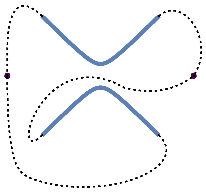
\includegraphics[width=\linewidth]{figures/projective-hyperbola-loop.pdf}}
如 Proposition~\ref{prop:projective-space-affine-plus-infinity} 后的讨论所示, 它们分别趋向 $\mathbb{P}^{2}$ 中的点 $[0:1:1]$ 和 $[0:1:-1]$. 如图所示, 沿着 $X_{0}$ 和两个无穷远点组成的路径走, 可以看到整个射影簇 $X$ 的实点组成一个环, 就像 $\mathbb{P}_{\mathbb{R}}^{1}$. 实际上, 讨论过射影簇的同构之后, 我们将看到存在同构 $X\cong\mathbb{P}_{\mathbb{C}}^{1}$.
\end{Example}

推广 Example~\ref{ex:affine-restriction-of-projective-conic}, 若 $X=\mathcal{V}_{\mathbb{P}}(S)\subseteq\mathbb{P}^{n}$ 为射影簇, 则
\[
  X=X_{0}\sqcup\{X\text{ 中的无穷远点}\},
\]
其中
\[
  X_{0}=\{[a_{0}:\cdots:a_{n}]\in X\mid a_{0}\neq0\},
\]
而 $X$ 中的无穷远点正是满足 $a_{0}=0$ 的那些点. 也就是说, 在 $\mathbb{A}^{n}$ 与 $\mathbb{P}^{n}$ 中第一个坐标非零的点之间的自然双射下, 有 $X_{0}=X\cap\mathbb{A}^{n}$. 由于 $X_{0}$ 中的点可写成 $[1:b_{1}:\cdots:b_{n}]$, 可见
\[
  X_{0}=\mathcal{V}_{\mathbb{A}}(S_{0})\subseteq\mathbb{A}^{n},
\]
其中
\[
  S_{0}=\{f(1,x_{1},\ldots,x_{n})\mid f\in S\}\subseteq K[x_{1},\ldots,x_{n}].
\]
特别地, $X_{0}$ 是仿射簇, 称为 $X$ 的\emph{仿射限制}. 再看一类例子.

\begin{Example}{$\mathbb{P}^{2}$ 中直线的仿射限制}\leavevmode\label{ex:affine-restrictions-of-projective-lines}
Example~\ref{ex:projective-line-in-projective-plane} 中射影簇 $X=\mathcal{V}_{\mathbb{P}}(x_{0}+x_{1}-x_{2})\subseteq\mathbb{P}^{2}$ 的仿射限制是直线 $X_{0}=\mathcal{V}_{\mathbb{A}}(1+x_{1}-x_{2})\subseteq\mathbb{A}^{2}$, 而 $X$ 唯一的无穷远点是 $[0:1:1]$. 更一般地, 射影簇
\[
  L=\mathcal{V}_{\mathbb{P}}(bx_{0}+mx_{1}-x_{2})\subseteq\mathbb{P}^{2}
\]
的仿射限制是
\[
  L_{0}=\mathcal{V}_{\mathbb{A}}(b+mx_{1}-x_{2})\subseteq\mathbb{A}^{2},
\]
即纵截距为 $b$, 斜率为 $m$ 的直线. 稍作思考可知, $L$ 仍只含一个无穷远点: $[0:1:m]$. 这使 Section~\ref{sec:projective-space} 的直观描述更精确了: $[0:1:m]$ 就是\textquotedbl{}沿 $L_{0}$ 走\textquotedbl{}所到达的无穷远点.

特别地, 沿 $L_{0}$ 走到的无穷远点只取决于 $L_{0}$ 的斜率. 因此, 平行直线, 例如
\[
  \mathcal{V}_{\mathbb{A}}(1+3x_{1}-x_{2}),\quad
  \mathcal{V}_{\mathbb{A}}(2+3x_{1}-x_{2})\subseteq\mathbb{A}^{2},
\]
在 $\mathbb{A}^{2}$ 中不相交, 但把它们看成射影直线
\[
  \mathcal{V}_{\mathbb{P}}(x_{0}+3x_{1}-x_{2}),\quad
  \mathcal{V}_{\mathbb{P}}(2x_{0}+3x_{1}-x_{2})\subseteq\mathbb{P}^{2}
\]
的仿射限制时, 它们相交于由共同斜率决定的无穷远点 $[0:1:3]$. 因此, 有时把 $\mathbb{P}^{2}$ 称为\textquotedbl{}平行线相交\textquotedbl{}的空间. 对这一现象更完整的探讨见 Exercise~\ref{ex:intersection-of-two-projective-lines}.
\end{Example}

上面让 $x_{0}$ 而不是其他变量起这个作用, 只是任意选择. 更一般地, 将射影簇限制到 $\mathbb{P}^{n}$ 中第 $i$ 个坐标非零的点, 会得到一个仿射簇. 具体见下列定义.

\begin{Definition}{仿射开片与仿射限制}\leavevmode\label{def:affine-patches-and-restrictions}
对每个 $i\in\{0,1,\ldots,n\}$, $\mathbb{P}^{n}$ 的\emph{第 $i$ 个仿射开片}是集合
\[
  \mathbb{A}_{i}^{n}=\{[a_{0}:a_{1}:\cdots:a_{n}]\in\mathbb{P}^{n}\mid a_{i}\neq0\},
\]
对任意集合 $X\subseteq\mathbb{P}^{n}$, 称交集 $X\cap\mathbb{A}_{i}^{n}$ 为 $X$ 的\emph{第 $i$ 个仿射限制}.
\end{Definition}

建议读者停下来验证 (Exercise~\ref{ex:affine-patch-bijection-and-restriction}): 对任意 $i$, 有自然双射 $\mathbb{A}_{i}^{n}=\mathbb{A}^{n}$, 在此双射下, $X=\mathcal{V}_{\mathbb{P}}(S)$ 的第 $i$ 个仿射限制是 $\mathcal{V}_{\mathbb{A}}(S_{i})\subseteq\mathbb{A}^{n}$, 其中
\[
  S_{i}=\{f(x_{0},\ldots,x_{i-1},1,x_{i+1},\ldots,x_{n})\mid f\in S\}.
\]

\begin{Example}{$\mathbb{P}^{2}$ 中一条三次曲线的仿射限制}\leavevmode\label{ex:affine-charts-of-projective-cubic}
考虑 $X=\mathcal{V}_{\mathbb{P}}(x_{0}x_{2}^{2}-2x_{1}^{3}-2x_{0}x_{1}^{2})\subseteq\mathbb{P}^{2}$ 的三个仿射限制:
\[
  \begin{aligned}
    X_{0}&=\mathcal{V}_{\mathbb{A}}(x_{2}^{2}-2x_{1}^{3}-2x_{1}^{2})\subseteq\mathbb{A}^{2},\\
    X_{1}&=\mathcal{V}_{\mathbb{A}}(x_{0}x_{2}^{2}-2-2x_{0})\subseteq\mathbb{A}^{2},\\
    X_{2}&=\mathcal{V}_{\mathbb{A}}(x_{0}-2x_{1}^{3}-2x_{1}^{2}x_{0})\subseteq\mathbb{A}^{2}.
  \end{aligned}
\]
整个射影簇 $X$ 是这三个子集的并; 坐标中有不止一个非零坐标的点属于这些子集的交. 因此, 可以把三个有大量重叠的仿射簇\textquotedbl{}粘合在一起\textquotedbl{}, 构造 $X$. 例如, 点 $[1:1:2]\in X$ 出现在这三个仿射限制中: 在 $X_{0}$ 中, 它的仿射坐标是 $(x_{1},x_{2})=(1,2)$; 在 $X_{1}$ 中, 它的仿射坐标是 $(x_{0},x_{2})=(1,2)$; 在 $X_{2}$ 中, 它的仿射坐标是 $(x_{0},x_{1})=(\frac{1}{2},\frac{1}{2})$. \hyperref[fig:projective-cubic-affine-charts]{下图}画出了实数域上的三个仿射限制. 每幅图中用颜色标出四个点, 同色点在 $X$ 中彼此认同. 箭头指示这些仿射限制粘合的方向.

{\centering\phantomsection\label{fig:projective-cubic-affine-charts}%
  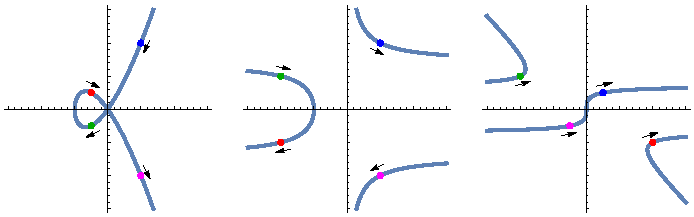
\includegraphics[width=.98\linewidth]{figures/projective-cubic-affine-charts.pdf}\par}

沿曲线仔细走一遍, 在必要时从一个仿射限制切换到另一个, 可以看出在实数域上, $X$ 构成一个\textquotedbl{}八字形\textquotedbl{}. 第一个仿射限制缺少一个点 (竖直直线上的无穷远点), 第二个和第三个各缺少两个点, 其中有一个点 (水平直线上的无穷远点) 是八字形的自交点.
\end{Example}

从射影簇 $X$ 到它的仿射限制, 只需将某个坐标设为 $1$. 但能否反过来操作? 也就是说, 从仿射簇 $X$ 出发, 能否找到一个射影簇 $\overline{X}$, 使 $X$ 是 $\overline{X}$ 的某个仿射限制? 答案是\textquotedbl{}能\textquotedbl{}, 相应的射影簇称为 $X$ 的\emph{射影闭包}, 这就是下一节的话题.

\BookExerciseHeading
\begin{BookExercises}
  \item\label{ex:intersection-of-two-projective-lines} $\mathbb{P}^{2}$ 中的直线是形如
  \[
    \mathcal{V}_{\mathbb{P}}(ax_{0}+bx_{1}+cx_{2})\subseteq\mathbb{P}^{2}
  \]
  的射影簇, 其中 $a,b,c\in K$ 不全为零. 本题设 $X$ 和 $Y$ 为 $\mathbb{P}^{2}$ 中两条不同的直线.
  \begin{enumerate}
    \item 证明存在一个仿射开片 $\mathbb{A}_{i}^{2}$, 使得仿射限制 $X_{i}$ 和 $Y_{i}$ 均非空.
    \item 不失一般性, 假设仿射限制 $X_{0}$ 和 $Y_{0}$ 在 $\mathbb{A}_{0}^{2}$ 中非空. 利用 $X$ 和 $Y$ 的定义方程, 描述 $\mathbb{A}^{2}$ 中的直线 $X_{0}$ 和 $Y_{0}$.
    \item 证明, 只要 $X_{0}$ 和 $Y_{0}$ 不平行, 就有 $X\cap Y=X_{0}\cap Y_{0}$.
    \item 证明, 当 $X_{0}$ 和 $Y_{0}$ 平行时, $X\cap Y$ 含有唯一的无穷远点.
  \end{enumerate}
  \item\label{ex:affine-patch-bijection-and-restriction}
  \begin{enumerate}
    \item 证明 $\mathbb{P}^{n}$ 中的仿射开片 $\mathbb{A}_{i}^{n}$ 与仿射空间 $\mathbb{A}^{n}$ 之间有自然双射.
    \item 若 $X=\mathcal{V}_{\mathbb{P}}(S)\subseteq\mathbb{P}^{n}$, 证明 (a) 中的双射将 $X\cap\mathbb{A}_{i}^{n}$ 与 $\mathcal{V}_{\mathbb{A}}(S_{i})\subseteq\mathbb{A}^{n}$ 认同, 其中
    \[
      S_{i}=\{f(x_{0},\ldots,x_{i-1},1,x_{i+1},\ldots,x_{n})\mid f\in S\}.
    \]
  \end{enumerate}
  \item\label{ex:three-affine-restrictions-of-a-parabola} 令 $X=\mathcal{V}_{\mathbb{P}}(x_{0}x_{2}-x_{1}^{2})\subseteq\mathbb{P}^{2}$.
  \begin{enumerate}
    \item 求三个仿射限制 $X_{0},X_{1},X_{2}$, 并画出它们在实数域上的图形.
    \item 考虑点 $(2,4)\in X_{0}\subseteq\mathbb{A}^{2}$. 作为 $X$ 的元素, 它是点 $[1:2:4]$, 这个点也属于 $X_{1}$. 这个点在 $X_{1}\subseteq\mathbb{A}^{2}$ 中的坐标是什么?
    \item 对 $X_{0}\cap X_{1}$ 中其他若干点重复 (b) 的推理, 以图示方式说明 $X_{0}$ 与 $X_{1}$ 如何在 $X$ 内拼合. 然后对 $X_{1}$ 与 $X_{2}$, 以及 $X_{0}$ 与 $X_{2}$ 也做同样的事.
  \end{enumerate}
  \item\label{ex:three-affine-restrictions-of-a-chosen-curve} 取 $X=\mathcal{V}(f)\subseteq\mathbb{P}^{2}$, 其中 $f\in K[x_{0},x_{1},x_{2}]$ 是你选取的一个齐次多项式, 重做上一题.
  \item\label{ex:affine-restrictions-of-real-projective-quadric} 画出 $X=\mathcal{V}(w^{2}+x^{2}+y^{2}-z^{2})\subseteq\mathbb{P}_{\mathbb{R}}^{3}$ 的四个仿射限制, 并描述它们如何拼合.
  \item\label{ex:affine-restrictions-of-real-split-projective-quadric} 画出 $X=\mathcal{V}(w^{2}+x^{2}-y^{2}-z^{2})\subseteq\mathbb{P}_{\mathbb{R}}^{3}$ 的四个仿射限制, 并描述它们如何拼合.
\end{BookExercises}
